%%%%%%%%%%%%%%%%%%%%%%%%%%%%%%%%%%%%%%%%%%%%%%%%%%%%%%%%%%%%%%%%%%%%%%%%%%%%%%%%
%                                                                              %
% ttH_H_to_bb_3                                                                %
%                                                                              %
% version: 2016-04-12T1316Z                                                    %
%                                                                              %
% Will Breaden Madden                                                          %
%                                                                              %
%%%%%%%%%%%%%%%%%%%%%%%%%%%%%%%%%%%%%%%%%%%%%%%%%%%%%%%%%%%%%%%%%%%%%%%%%%%%%%%%
%                                                                              %
% DESCRIPTION                                                                  %
%                                                                              %
% This program produces a Feynman diagram.                                     %
%                                                                              %
%%%%%%%%%%%%%%%%%%%%%%%%%%%%%%%%%%%%%%%%%%%%%%%%%%%%%%%%%%%%%%%%%%%%%%%%%%%%%%%%
%                                                                              %
% LICENCE INFORMATION                                                          %
%                                                                              %
% This program produces a document.                                            %
%                                                                              %
% copyright (C) 2016 William Breaden Madden                                    %
%                                                                              %
% This software is released under the terms of the GNU General Public License  %
% version 3 (GPLv3).                                                           %
%                                                                              %
% This program is free software: you can redistribute it and/or modify it      %
% under the terms of the GNU General Public License as published by the Free   %
% Software Foundation, either version 3 of the License, or (at your option)    %
% any later version.                                                           %
%                                                                              %
% This program is distributed in the hope that it will be useful, but WITHOUT  %
% ANY WARRANTY; without even the implied warranty of MERCHANTABILITY or        %
% FITNESS FOR A PARTICULAR PURPOSE.  See the GNU General Public License for    %
% more details.                                                                %
%                                                                              %
% For a copy of the GNU General Public License, see                            %
% <http://www.gnu.org/licenses/>.                                              %
%                                                                              %
%%%%%%%%%%%%%%%%%%%%%%%%%%%%%%%%%%%%%%%%%%%%%%%%%%%%%%%%%%%%%%%%%%%%%%%%%%%%%%%%

\documentclass[tikz]{standalone}

\usepackage[compat=1.1.0]{tikz-feynman}

\begin{document}
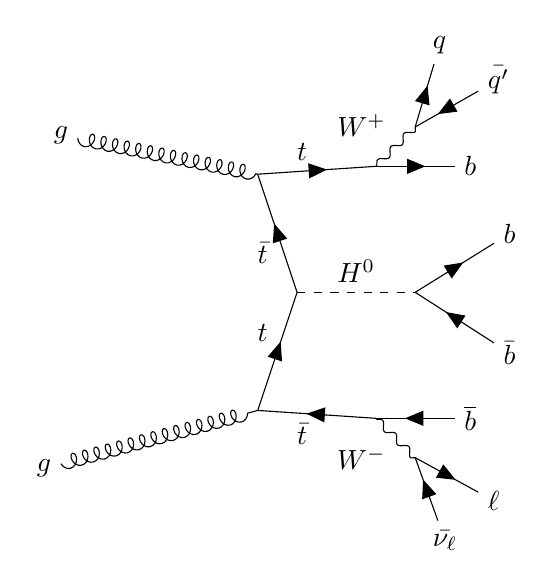
\begin{tikzpicture}
    \begin{feynman}
        % g, t
        \vertex (g1) {\({g}\)};
        \vertex[below right=0.5cm and 2.5cm of g1] (t4);
        \vertex[below right=1.5cm and 0.5cm of t4] (t3);
        \vertex[below left=1.5cm and 0.5cm of t3] (t2);
        \vertex[below left=0.5cm and 2.5cm of t2] (g2) {\({g}\)};
        
        \vertex[above right=0.1cm and 1.5cm of t4] (t5);
        \vertex[below right=0.1cm and 1.5cm of t2] (t1);
        
        % upper shower
        \vertex[right=1cm of t5] (f3) {\({b}\)};
        \vertex[above right=0.5cm and 0.5cm of t5] (W1);
        \vertex[above right=0.8cm and 0.1cm of W1] (f1) {\({q}\)};
        \vertex[above right=0.3cm and 0.8cm of W1] (f2) {\({\bar{q^{\prime}}}\)};
        
        % lower shower
        \vertex[right=1cm of t1] (f6) {\(\overline b\)};
        \vertex[below right=0.5cm and 0.5cm of t1] (W2);
        \vertex[below right=0.8cm and 0.1cm of W2] (f7) {\({\bar{\nu_{\ell}}}\)};
        \vertex[below right=0.3cm and 0.8cm of W2] (f8) {\({\ell}\)};
        
        % H
        \vertex[right=1.5cm of t3] (H);
        \vertex[above right=0.5cm and 1cm of H] (f4) {\({b}\)};
        \vertex[below right=0.5cm and 1cm of H] (f5) {\({\bar{b}}\)};
        
        \diagram*{
            (g1) -- [gluon] (t4),
            (g2) -- [gluon] (t2),
            {[edges=fermion] 
                (f6) -- (t1) 
                     -- [edge label=\({\bar{t}}\)] (t2) 
                     -- [edge label=\(t\)] (t3) 
                     -- [edge label=\({\bar{t}}\)] (t4) 
                     -- [edge label=\(t\)] (t5) 
                     -- (f3),
                (f7) -- (W2) -- (f8),
                (f2) -- (W1) -- (f1),
                (f5) -- (H) -- (f4),
            },
            (t3) -- [scalar, edge label=\({H^{0}}\)] (H),
            (t1) -- [boson, edge label'=\({W^{-}}\)] (W2),
            (t5) -- [boson, edge label=\({W^{+}}\)] (W1),
        };
    \end{feynman}
\end{tikzpicture}
\end{document}
